\documentclass[../Article_Sensitivity_Analsysis.tex]{subfiles}
\graphicspath{{\subfix{../Figures/}}}
\begin{document}
	
    %\subsection{Pressure}
	
	As discussed in Chapter \ref{CH:Governing_equations_chapter}, a small pressure wave propagates at the speed of sound relative to the flow. If the flow velocity is relatively low, all pressure changes are hydrodynamic (resulting from velocity motion) rather than thermodynamic. The Low Mach number assumption leads to instant propagation of the thermodynamic pressure throughout the system and allows for considering a single pressure value for the entire system. The local sensitivity analysis results can be interpreted as a system response to the step-change (deviation) of the pressure. 
	
	\begin{comment}
	\begin{figure}[h!]
		\centering
		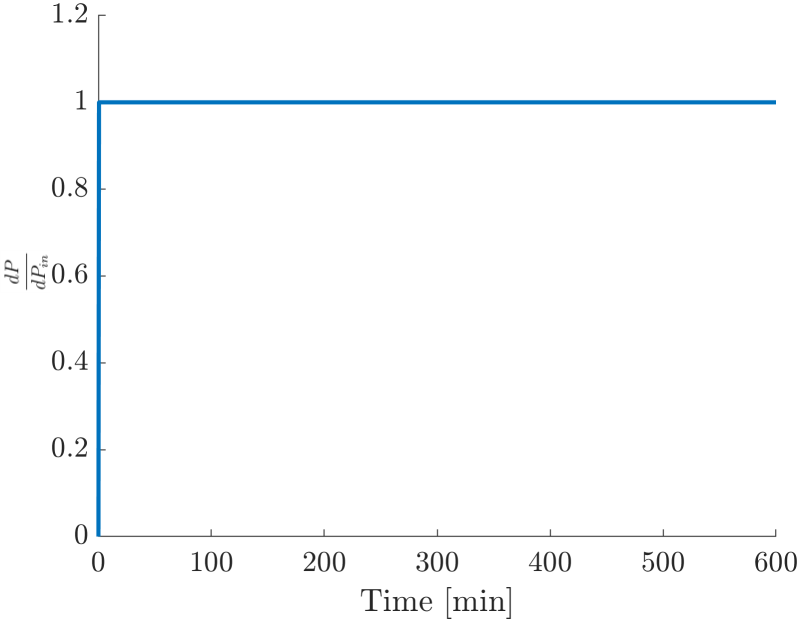
\includegraphics[trim = 0.0cm 0.0cm 0.0cm 0.0cm,clip,width=\columnwidth]{/Results_sensitivity/P_P_1.png}
		\caption{The effect of $P_{in}$ change on $P$}
		\label{fig:Sensitivty_P_P}
	\end{figure}
	\end{comment}
	
	In response to the pressure change, the energy equation experiences a deviation in the whole spatial domain simultaneously. The pressure change affects the fluid's temperature inside the computational domain, but boundary values are subject to constraints specified at the extremes of that domain. Applying the Dirichlet boundary conditions imposes a fixed temperature value at the inlet, which leads to a thermal gradient propagating along the system. In contrast, Neumann boundary conditions dictate the heat flux at the boundaries. In this work, Neumann boundary conditions of zero were used to ensure that the temperatures at the inlet, outlet, and inside the extractor would vary uniformly and according to the pressure change.
	
	\begin{comment}
	\begin{figure}[h!]
		\centering
		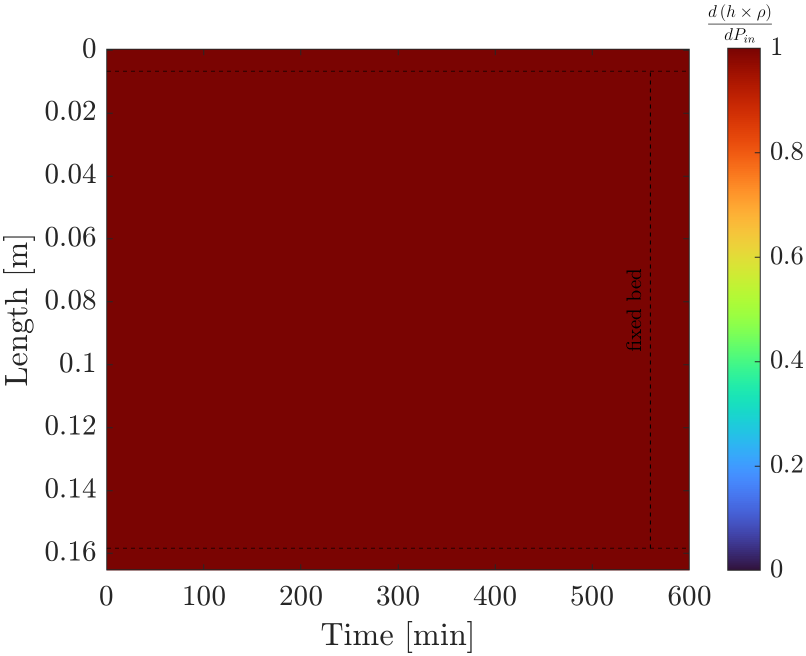
\includegraphics[trim = 0.0cm 0.0cm 0.0cm 0.0cm,clip,width=\columnwidth]{/Results_sensitivity/H_P_1.png}
		\caption{The effect of $P_{in}$ change on $(h \times \rho)$}
		\label{fig:Sensitivty_P_H}
	\end{figure}
	\end{comment}
	
	Figure \ref{fig:Sensitivty_P_CS} shows the sensitivity of the solute concentration in the solid phase in response to pressure change. As discussed in Chapter \ref{CH: Continuity}, the velocity of a fluid is inversely proportional to its density, which suggests that the pressure reduces the fluid's velocity. As a result, the residence time is extended, causing longer interaction between the solute and solvent. Initially, the extraction process is in the kinetic-controlled regime, where the concentration gradient is high, and the limiting factor is the solute solubility. As discussed in {\color{red}article 1}, the system is considered to be far from saturation, which explains the low system response at the beginning of the process. In the sensitivity analysis of \citet{Fiori_2007}, the low initial system response was also observed. The system response becomes evident when the concentration gradient diminishes, and the extraction switches from the kinetic-controlled to the diffusion-controlled regime. The negative sign is interpreted as a faster solute loss from the solid phase, which corresponds to enhanced mass transfer. Over time, the amount of solute becomes a limiting factor, and the pressure change effect on the system is reduced. Eventually, the sensitivities approach zero asymptotically when the solute is washed out from the solid bed.

	\begin{figure}[!ht]
		\centering
		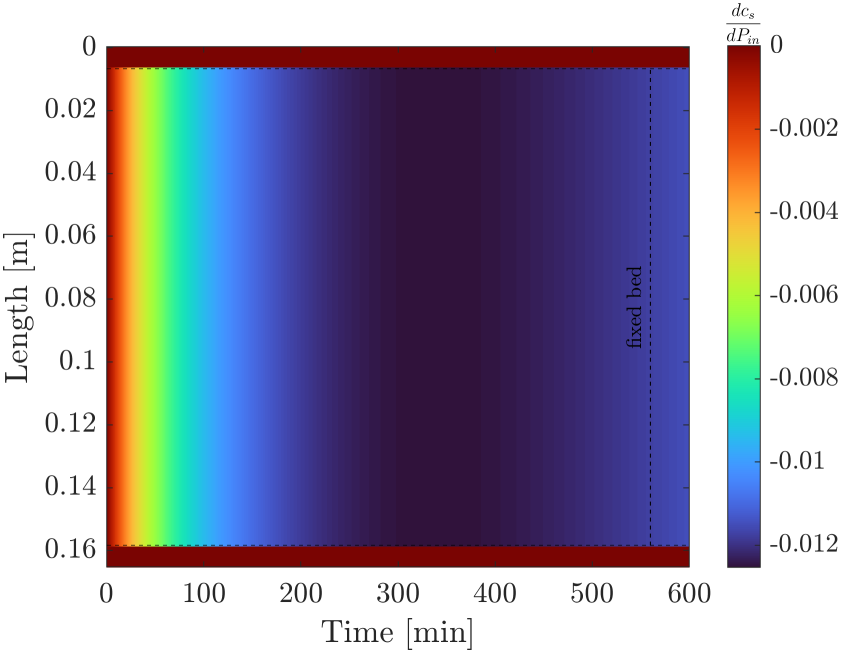
\includegraphics[trim = 0.0cm 0.0cm 0.0cm 0.0cm,clip,width=\columnwidth]{/Results_sensitivity/CS_P_1.png}
		\caption{The effect of $P_{in}$ change on $C_s$}
		\label{fig:Sensitivty_P_CS}
	\end{figure}
	
	Figure \ref{fig:Sensitivty_P_CF} shows how sensitive is the solute concentration in the fluid phase to the pressure change. Compared to Figure \ref{fig:Sensitivty_P_CS}, the dynamic behaviour of the fluid phase sensitivities can be observed. Due to the advection, the sensitivities move along the system analogously to the solute in the fluid phase. Although the pressure increase improves the mass transfer, the system response is initially low, which reflects the idle period discussed above. Later, the sensitivities increase due to faster solute loss from the solid phase. The positive sensitivities indicate that more solute is transported from the particles to the fluid. When the amount of solute in the solid phase becomes a limiting factor, the extraction rate slows down, and sensitivities decline to negative values and eventually goes asymptotically towards zero.
	
	\begin{figure}[!ht]
		\centering
		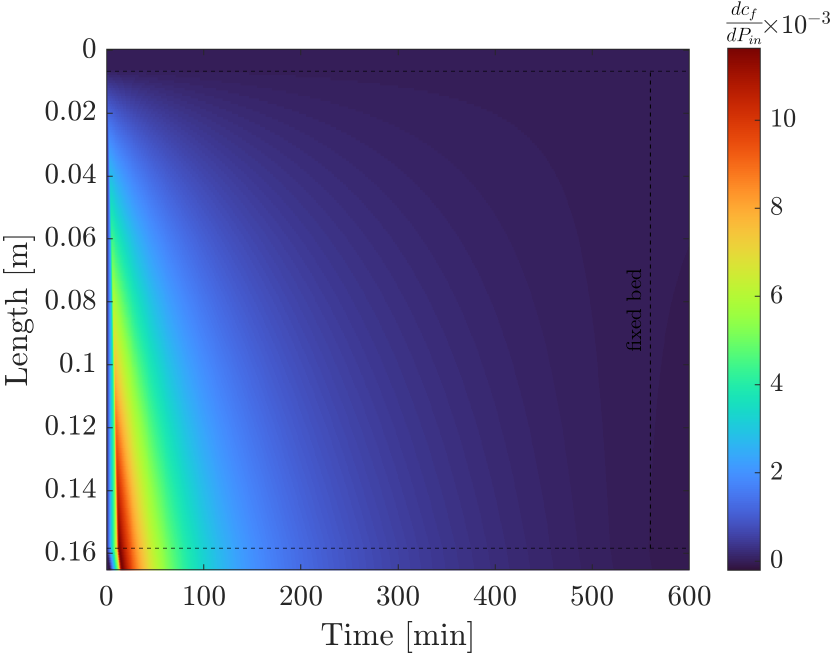
\includegraphics[trim = 0.0cm 0.0cm 0.0cm 0.0cm,clip,width=\columnwidth]{/Results_sensitivity/CF_P_1.png}
		\caption{The effect of $P_{in}$ change on $C_f$}
		\label{fig:Sensitivty_P_CF}
	\end{figure}
	
	Figure \ref{fig:Sensitivty_P_y} illustrates how sensitive the extraction yield is to the pressure changes. The effect of pressure change on the yield is expanded and consider for multiple values of pressure. Initially, all the sensitivity curve stay almost flat, suggesting a latency in the system's response. Due to the decreased velocity of the fluid, the solute reaches the extractor's outlet later, which causes minor negative sensitivities to appear. When the solute reaches exits the extractor, the sensitivity curves increase rapidly. The positive yield sensitivities indicate improved process efficiency, which is directly related to enhanced mass transfer. The peak in $\frac{dy}{dP_{in}}$ reflects when the deviation from the original system is the largest. Eventually, the sensitivities decline and converge towards zero. The concentration gradient becomes a limiting factor, and the enhanced mass transfer no longer plays a dominant role compared to the original system. It can be observed that the yield is more sensitivity at low pressure. 
	
	\begin{figure}[!ht]
		\centering
		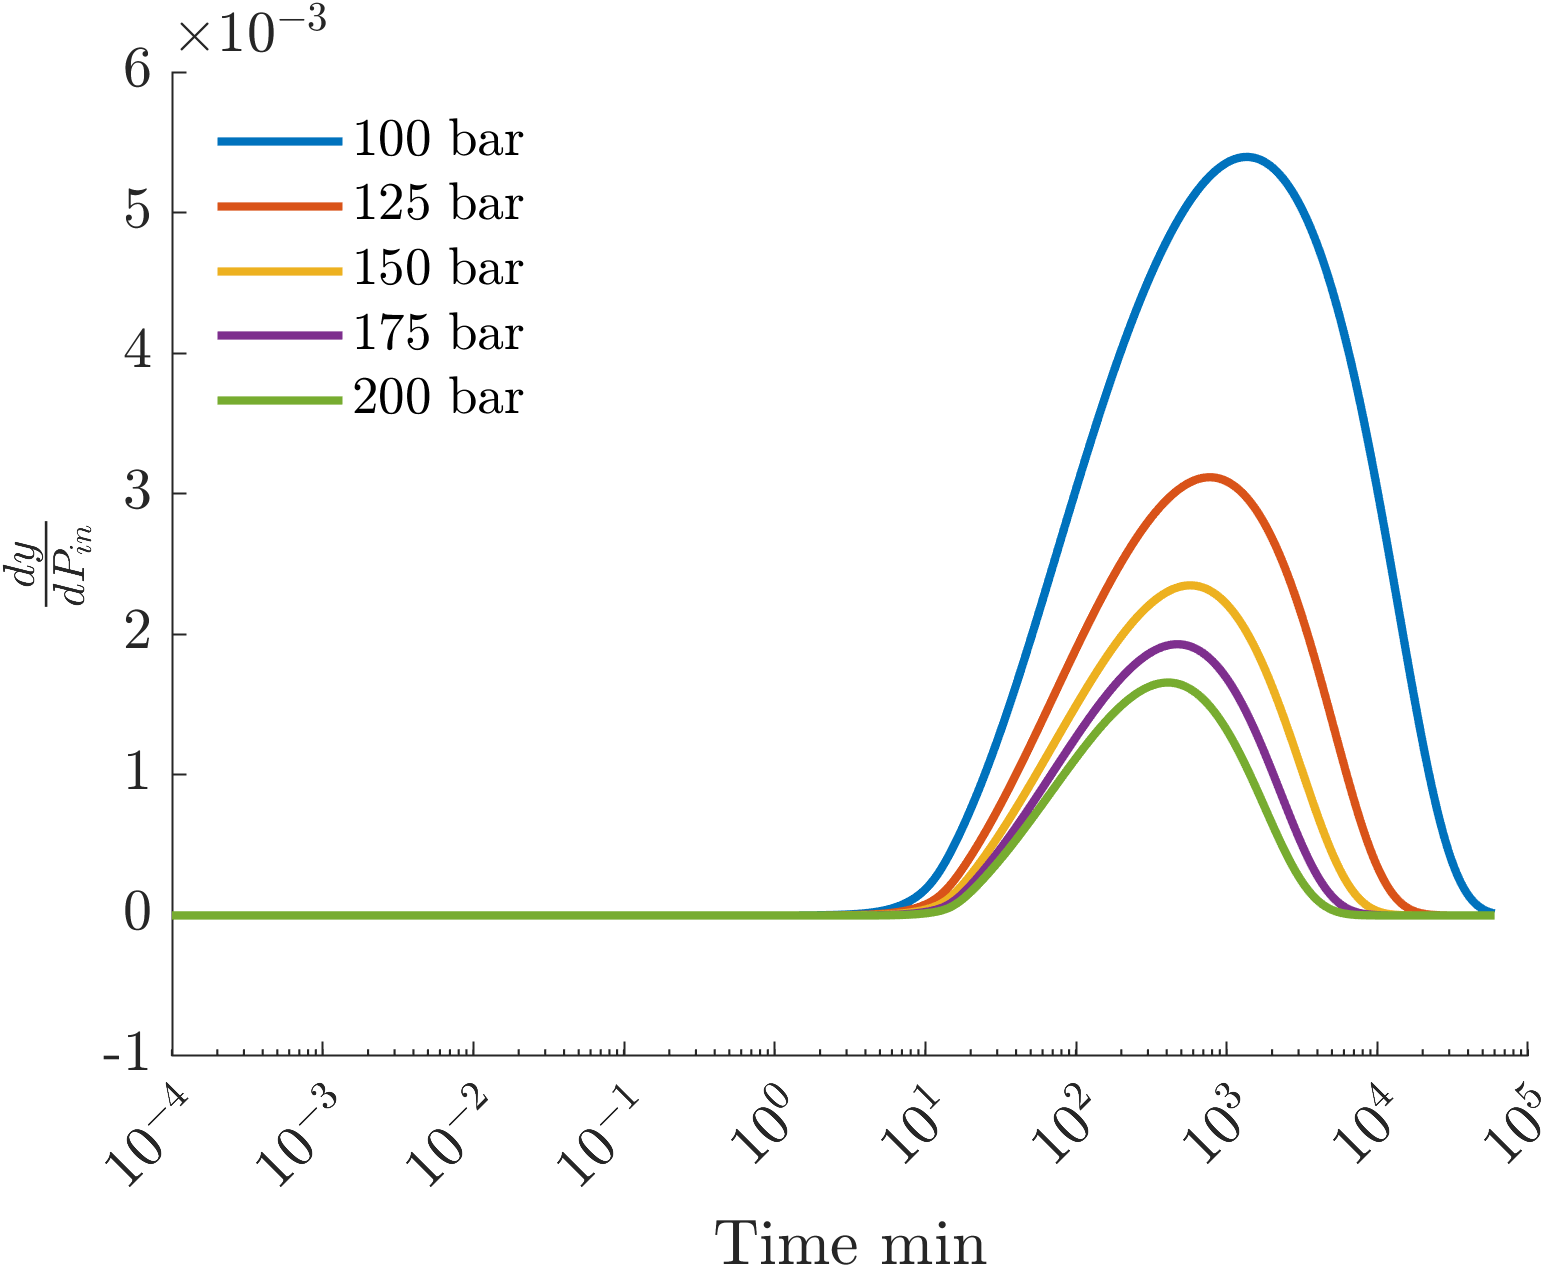
\includegraphics[trim = 0.0cm 0.0cm 0.0cm 0.0cm,clip,width=\columnwidth]{/Results_sensitivity/Yield_Multiple.png}
		\caption{The effect of $P_{in}$ change on $y(t)$}
		\label{fig:Sensitivty_P_y}
	\end{figure}
		
\end{document}


































